\documentclass{article}
\usepackage{amsmath}
\usepackage{indentfirst}
\usepackage{graphicx}
\usepackage[square]{natbib}
\usepackage{caption}
\usepackage{hyperref}
\usepackage{xcolor}
\usepackage{subcaption}
\newcommand{\highlight}[1]{%
  \colorbox{red!50}{$\displaystyle#1$}}
\usepackage{tcolorbox}
\newcommand\tenpow[1]{\ensuremath{{\times}10^{#1}}}
\newcommand\und{\textunderscore}
% These are the package Aurelien uses
\usepackage[top=2cm,bottom=2cm,right=2.5cm,left=2.5cm]{geometry}
\begin{document}
\title{Analysis of The Rothermel Model in Two Fire Spread Models (WFA and WRF-SFIRE)}
\author{By: Jeremy Benik, Adam Kochanski, Angel Farguell Caus}
\maketitle


\section{Introduction}
	This document will outline the key differences between the Rothermel model implementation in WRF-SFIRE and the Rothermel model implementation in WFA. WRF-SFIRE's implementation of Rothermel is based on the CAWFE code whereas the WFA Rothermel model is based on Patricia L. Andrew's paper. This paper is developed on the "consideration of how each fuel parameter within the model exerts its effect on the three characteristic features of a spreading fire: energy source, energy sink, and flow of air or heat within the array"\citep{Andrews2018}. 
	
	For this analysis, the final rate of spread (ROS) equations from both models will be analyzed initially to discuss the major differences, and then each component with major differences will be further discussed and analyzed. The first part will be analyzing the no slope and no wind component, and then the slope and wind coefficients will be added in after the initial analysis. 
	
	To accurately test the models, both models used the same input parameters (fuel type 1 (short grass), 3\% FMC, 0 wind, 0 slope). This way we can see where the models diverge from each other. 
	
\section{Rothermel Model From WFA and WRF-SFIRE}

Here are the final equations from both models with the values so we can see the final calculation. 

% WFA Rothermel model
\subsubsection*{WFA}
	\begin{equation}
	\label{r0_WFA_2}
	\begin{split}
	r_0 &= \frac{ir * xifr}{heat\und sink\und dead + heat\und sink\und live} * 0.00508 \\
	0.0297 &= \frac{939.3928 * 0.0578}{0.0340 * 0.9613 * 283.4800} * 0.00508
	\end{split}
\end{equation}

\noindent Where: \\
r$_0$ = Rate of spread under no slope and no wind conditions \\
ir = Reaction intensity (btu/ft$^2$) \\
xifr = Propagating flux ratio \\
heat\und sink\und dead = Heat sink of the dead fuel \\
heat\und sink\und live = Heat sink of the live fuel
% WRF-SFIRE model
\subsubsection*{WRF-SFIRE}
\begin{equation}
	\label{WRF-ROS}
	\begin{split}
		r_0 &= \frac{ir*xifr}{rhob * epsilon *qig} * .00508 \\
		0.0265 &= \frac{812.8685 * 0.0577}{0.0330 * 0.9613 * 283.4800} * 0.00508
	\end{split}
\end{equation}
\noindent Where: \\
r$_0$ = Rate of Spread under no slope and no wind conditions \\
ir = Reaction intensity (btu/ft$^2$) \\
xifr = Propagating flux ratio \\
rhob = Ovendry bulk density (lb/ft$^3$) \\
epsilon = Effective heating number \\
qig = heat of preignition (btu/lb)\\

The most notable difference here is ir. In WFA, the value for ir (939.3928) is much greater than in the WRF-SFIRE model (812.8685). Below is the calculation for ir for both models 


\subsubsection{IR (Reaction Intensity, $\frac{btu}{ft^2}$)}
Here are the reaction intensities from both WFA and from WRF-SFIRE. 

WFA: 
\begin{equation}
\label{WFA_IR_2}
\begin{split}
		ir &= gamma * (wn\und dead * fuelheat\und dead * etam\und dead * etas\und dead + \\
		& wn\und live * fuelheat\und live * etam\und live * etas\und live) \\
        939.3928 &= 14.2014 * (0.0321 * 8000 * 0.6169 * 0.4174 + 0 + 0 + 0 + 0)
\end{split}
\end{equation}
	
WRF-SFIRE:
\begin{equation}
\label{IR_WRF_2}
	\begin{split}
		ir       &= gamma * wn * fuelheat * etam * etas \\
		812.8685 &= 13.4642 * 0.0313 * (7.4962 \tenpow{3}) * 0.6169 * 0.4147
	\end{split}
\end{equation}


As we can see, these two parameters differ from each other by quite a significant amount. The biggest difference between the two equations are the values for gamma and the fuelheats. The fuelheat is an input parameter from the fuels file and it varies between these two models. In WFA, the fuelheat is set to 8000 BTU/lb and the fuelheat in WRF-SFIRE is 7496.2 BTU/lb. By modifying the fuelheat parameter in WFA to have the same value as WRF-SFIRE, we get an ir of 880.2345 which is still significantly larger that the calculation in WRF-SFIRE. To better understand what is leading to these differences, we went through the calculations for gamma to find what is causing these differences in the calculation. These calculations can be seen in equations \ref{gamma_WFA} and equations \ref{gamma_WRF}
\subsubsection{Gamma}


WFA
\begin{equation}
	\label{gamma_WFA}
	\begin{split}
		\Gamma &= gammax*(ratio^a * \exp(a*(1.-ratio)) \\
		14.2014 &= 16.1837 * 0.2534 ^ {0.2087} * e^{0.2087 * (1 - 0.2534)} \\
		gammax &= rtemp2/(495. + 0.0594*rtemp2) \\
		16.1837 &= 2.0706\tenpow{5} (495 + 0.0594* 2.0706\tenpow{5}) \\
		ratio &= betafl/betaop \\
		0.2534 &= 0.0011 / 0.0042 \\
		betafl &= fuelload/(fueldepth * fueldens) \\
		0.0011 &= 0.0340 / (1 * 32) \\
		fuelload &= \Sigma fuelloads \\ 
	    a &= 133 * savr ^ {-0.7913} \\
		0.2087 &= 133 * 3500^{-0.7913} 
	\end{split}
\end{equation}


WRF-SFIRE
\begin{equation}
\label{gamma_WRF}
	\begin{split}
		\Gamma &= gammax*(ratio^a)*\exp(a*(1.-ratio)) \\
		13.4642 &= 16.1837 * (0.2459 ^ {0.2836}) * e^{0.2836 * (1- 0.2459)} \\
		gammax &= rtemp2/(495. + 0.0594*rtemp2) \\
		16.1837 &= 2.0706 \tenpow{5} / (495. + 0.0594* 2.0706 \tenpow{5}) \\
		ratio &= betafl / betaop \\
		0.2459 &= 0.0010 / 0.0042 \\
		betafl &= fuelload/(fueldepth * fueldens) \\
		0.0010 &= 0.0330 / (1.0007 * 32) \\
		a &= 1./(4.774 * savr^{0.1} - 7.27) \\
		0.2836 &= 1./(4.774 * 3500^{0.1} - 7.27)
	\end{split}
\end{equation}

The major differences between these calculations for gamma are the calculation for the coefficient for optimum reaction velocity (a). WRF-SFIRE uses the equation from the original Rothermel paper, however WFA uses a different equation taken from Andrews that yields a different value for this coefficient. By modifying the WFA model and forcing a to equal 0.2836, the resulting ROS is the same as the WRF-SFIRE calculation, indicating this parameter has a huge influence on the final ROS. 

\section{Different Fuel Classes}
Another difference among the models are WFA incorporates different fuel class parameters into the model whereas WRF-SFIRE only uses one value to represent the fuel. There are many places WFA uses the different classes for the calculation of the ROS, and they impact the model significantly. 

\subsubsection{Fuel Load}
 The first is the calculation for the total fuel load (lb/ft$^2$). WFA adds all the fuel loads together but this total fuel load is only used in the calculation for rhob and betafl (packing ratio). WFA uses the different fuel loads to calculate the mean total surface area per unit fuel cell (A\und *), weighting factors of each size class within each category, net fuel loading of each size class within each category (wn\und *), and the calculation live fuel moisture of extinction (exp**). The mean total surface area per unit fuel cell is then used to calculate weighting factors for each fuel class. These weighting factors are based on a "concept that a singular characteristic parameter can be found by weighting the variations in the parameter across the heterogeneous mixture" \citep{Andrews2018}. By weighting the fuels, this will give the most influence to the finer fuels \citep{Andrews2018}. 

 
 Comparing the two models, the total fuel load for fuel class 7 (Southern Rough) in WFA is 0.2240, but the fuel load in WRF-SFIRE for the same fuel type is 0.2172. With bigger fuels, there are more classes for that fuel category compared to finer fuels. With more classes of fuels, this will add an extra weighting parameter to the final calculation. 
 
\subsubsection{Surface Area to Volume Ratio (SAVR)}
Another fuel parameter with multiple classes is the SAVR. WFA uses the multiple classes in their calculations of: mean total surface area per unit fuel cell, weighting factors of each size class within each category, fuel particle surface-to-volume ratio of the dead and live categories, live fuel moisture of extinction, and the effective heating number of each size class within each category. WRF-SFIRE only uses one value for the SAVR. Like with the fuelload, the larger fuels have more classes for the SAVR compared to the finer fuels which typically have one or two classes. 

\subsubsection{Fuel Moisture Content (FMC)}
The last parameter with multiple classes is the fuel moisture. This is an input parameter for both of the models since the FMC changes with time. WFA uses the multiple FMC values in their calculations of: live fuel moisture of extinction, fuel moisture content of the dead and live categories, and the heat of preiginition of each size class within each category. WRF-SFIRE only uses one FMC value for each fuel. 

\section{fuel\und sink\und dead and fuel\und sink\und live}
The next difference between the models is the final calculation for the ROS. In equation \ref{r0_WFA_2} and equation \ref{WRF-ROS}, the denominator is different. In WFA, they add the head sink dead and live categories together whereas WRF-SFIRE uses the same calculation as the original Rothermel paper. These heat sink dead and alive parameters contain the same equations as the WRF-SFIRE ROS denominator, however they include the weighting factors, effective heating number of each size class within each category, and heat of preiginition of each size class within each category. The equations for heat sink dead and alive can be seen in equation \ref{heat_sink}:

\begin{equation}
	\label{heat_sink}
	\begin{split}
	heat\und sink\und dead &= rhob * f\und dead * ( f\und 1 * epsilon\und 1 * qig\und 1 + \\
	&f\und 10 * epsilon\und 10 * qig\und 10 + \\
	&f\und 100 * epsilon\und 100 * qig\und 100 + f\und herba\und dead \\
	&* epsilon\und herba\und dead * qig\und herba\und dead) \\
	heat\und sink\und live   &= rhob * f\und live * (f\und herba * epsilon\und herba * \\
    &qig\und herba +
    f\und woody * epsilon\und woody * qig\und woody)
	\end{split}
\end{equation}

 WRF-SFIRE only uses one value for the heat of preignition and the effective heating number for the final calculation whereas WFA uses the multiple classes as well as the weighting factors for each calculation. In fuels without multiple classes (such as fuel type 1), the denominator is close to the same (as seen in equation \ref{r0_WFA_2} and equation \ref{WRF-ROS}) since the weighting factors have no influence on the outcome (they are equal to 1 with fuel type 1 (short grass)) and there is no 10hr, 100hr, herbaceous, or woody component to that fuel. When a fuel with those parameters is used in the WFA model (such as Southern Rough), then the denominator would quickly diverge from the WRF-SFIRE model since the weighting factors and different classes would influence the outcome. 
 
 
 \section{Wind and Slope}
 
 The equations to calculate the wind and slope parameters differ slightly between both models as well. WFA incorporates both the total SAVR and fuelload for their calculation whereas WRF-SFIRE just uses the single value. The other major difference between the models is how the wind speed is input into the model. In WFA, there is a limit to how strong the winds can get before the model caps it off. This cap is based off the reaction intensity. If the reaction intensity multiplied by a coefficient is less than the wind speed, then the model will use that value instead of the input wind speed. WRF-SFIRE has a set cap at 30m/s so if the winds exceed that, then the model will use 30m/s. An example of how this influences the models can be seen in Figure 1 and Figure 2 where the ROS is no longer influenced by the wind speed in Figure 1 whereas the wind speed still influences the ROS in Figure 2. 

\begin{figure}[h]
\begin{minipage}{0.45\linewidth}
\label{WFA_ROS_2}
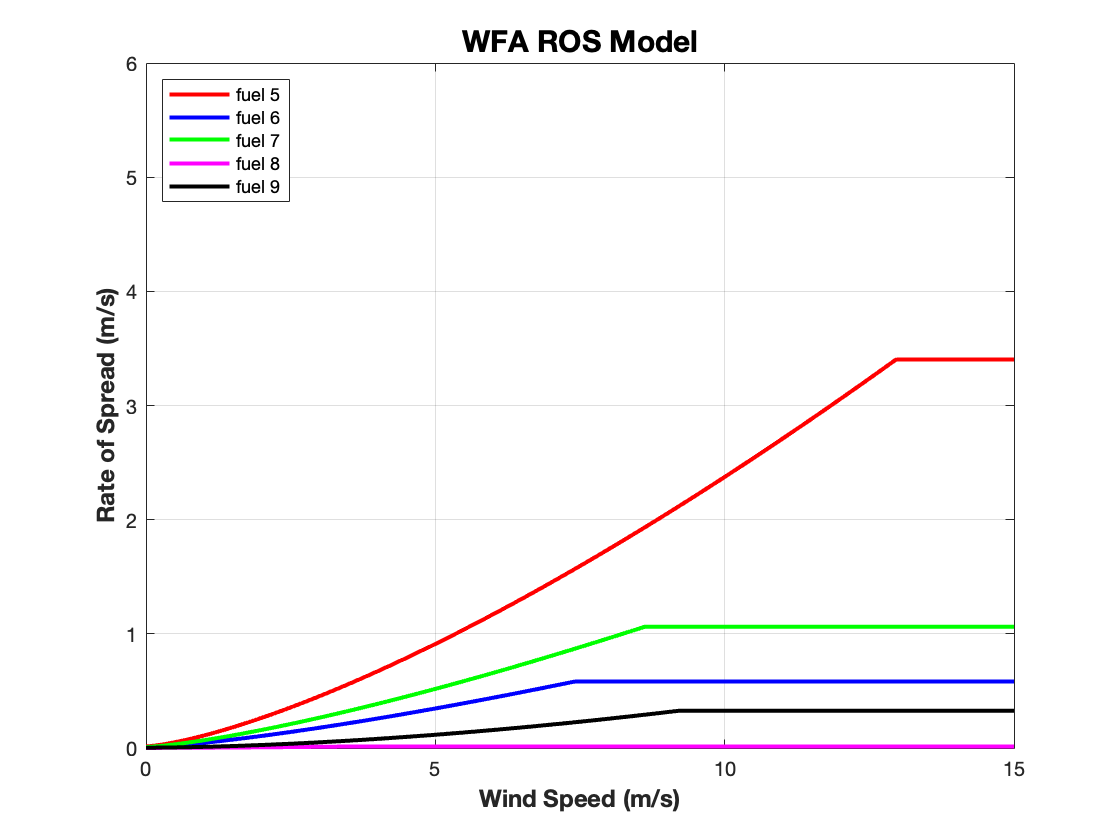
\includegraphics[width=\linewidth]{image_1.png}
\caption{WFA ROS calculations for fuel types 5-9}
\end{minipage}
\hfill
\begin{minipage}[c]{0.45\linewidth}
\label{WRF_ROS_2}
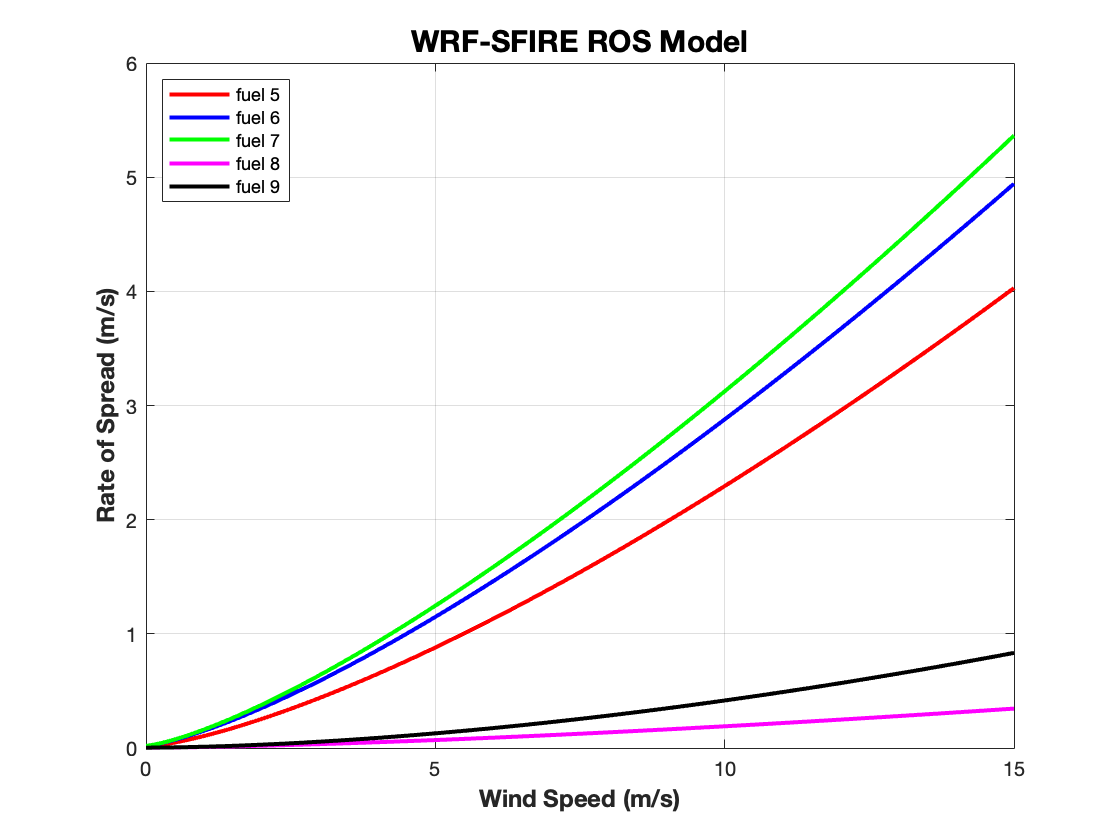
\includegraphics[width=\linewidth]{image_2.png}
\caption{WRF-SFIRE ROS calculations for fuel types 5-9}
\end{minipage}
\end{figure}
 

The slope parameter is calculated the same way between the models with the exception of WFA including the total fuelload for all size classes compared to WRF-SFIRE which uses one value for the fuel load. 
\section{Conclusion}
The WFA model and WRF-SFIRE model both aim to calculate the ROS of a propagating fire. However in the WFA model, they incorporate fuel classes for each fuel type which make the model much more complex compared to the WRF-SFIRE Rothermel model which only uses a single value for each fuel parameter. There are also differences in the calculation of the ROS in both models which makes the output ROS different even in cases where the fuel type only has dead 1hr properties in no slope and no wind conditions. Under slope and wind conditions the models also behave different with the WFA model artificially stopping the wind speed at a certain point whereas WRF-SFIRE has a set cap to the wind speed at 30m/s. 


\newpage
\bibliographystyle{agsm}
\bibliography{WFA_WRFSFIRE}


\end{document}

